% Saved into the git report.tex at 2017/12/15 at 00:11 from this web
\documentclass[a4paper]{article}
\usepackage[utf8]{inputenc}
%\usepackage{pythonhighlight}

\usepackage{graphicx}
\graphicspath{{fig/}}
\usepackage{color}
\usepackage{float}

% Click on references
\usepackage{hyperref}

% Use better tables
\usepackage{booktabs}

% Units
\usepackage{siunitx}

\usepackage{minted}
\newminted{py}{%
%		linenos,
		fontsize=\footnotesize,
		tabsize=4,
		mathescape,
}
\newminted{text}{%
%		linenos,
		fontsize=\small,
		tabsize=2,
		mathescape,
}

\title{Lab 6 - CSN: Network dynamics}
\author{Pierre-Antoine Porte \\ \texttt{porte.pierreantoine@gmail.com}
\and Rodrigo Arias Mallo \\ \texttt{rodarima@gmail.com}}
\date{\today}

%%% \def\arraystretch{1.5}

\begin{document}

\maketitle

\section{Introduction} % {{{1
%
In this session, we are going to generate some data by using 3 different
variations of the dynamical principles in Barabasi-Albert models (BA models in
the future).  Those principles are: vertex growth and preferential attachment.
The different variations of models we will implements are:
%
\begin{itemize}
	\item \textbf{A}: Vertex growth and preferential attachment (original).
	\item \textbf{B}: Vertex growth and uniform random attachment.
	\item \textbf{C}: Suppressed growth and preferential attachment.
\end{itemize}
%
Those generator models were simulated and the stored data will let us to analyze
mathematical properties. In this report we will show, discuss and explain the
results as well as the details of the implementation.
%
\section{Results} %{{{1
%
For each BA model (A, B and C), two metrics are analyzed, the distribution of 
the degrees of the nodes, and the evolution of a node as the graph grows over 
time.  We track the evolution of 4 different nodes selected from different 
points in the simulation. In the figures from~\ref{fig:best_dd_A} 
to~\ref{fig:bestC_dt1000} the best models are plotted along with the data. The 
notation for each model has been slightly changed, to avoid confusion. All 
models from session 2 where renamed with a T as prefix, and those from the 
session 3 a D as prefix instead. Those prefixes let us distinguish between say 
the model $D1$ and $T1$, as one is modeling the degree distribution, and the 
other the degree over time. The models for the evolution of degree over time can 
be shown in table~\ref{tab:Tmodels}, the models for the degree distribution are 
used in the minimum log likelihood form, and the only change is $\gamma = 3 $ in 
model 2 (see table 2 of session 2).
%
The tables~\ref{tab:AICdd} to~\ref{tab:AICdt1000} use AIC to
measure $\Delta = AIC - AIC_{best}$ of each model.
%
\begin{table}[H]
	\centering
	\begin{tabular}{cll}
		\toprule
		Model & Function & Parameters\\
		\midrule
		T0  & $f(n) = at$								& $a$ \\
		T1  & $f(t) = (t/2)^b$					& $b$ \\
		T2  & $f(t) = at^b$ 						& $a,b$\\
		T3  & $f(t) = ae^{ct}$					& $a,c$\\
		T4  & $f(t) = a\log t$					& $a$\\
		T5  & $f(t) = at^be^{ct}$				& $a,b,c$\\
		T1+ & $f(t) = (t/2)^b + d$			& $b,d$\\
		T2+ & $f(t) = at^b + d$					& $a,b,d$\\
		T3+ & $f(t) = ae^{ct} + d$			& $a,c,d$\\
		T4+ & $f(t) = a\log t + d$			& $a,d$\\
		T5+ & $f(t) = at^be^{ct} + d$	& $a,b,c,d$\\
		\bottomrule
	\end{tabular}
	\caption{The list of models to fit the degree over time.}
	\label{tab:Tmodels}
\end{table}

\newpage

\begin{figure}[H]
		\centering
		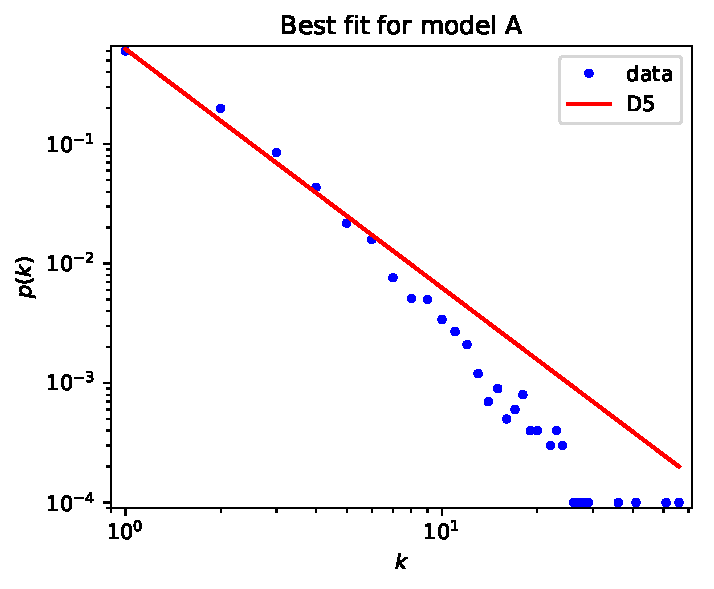
\includegraphics[width=0.45\textwidth]{modelA/best_dd.pdf}
		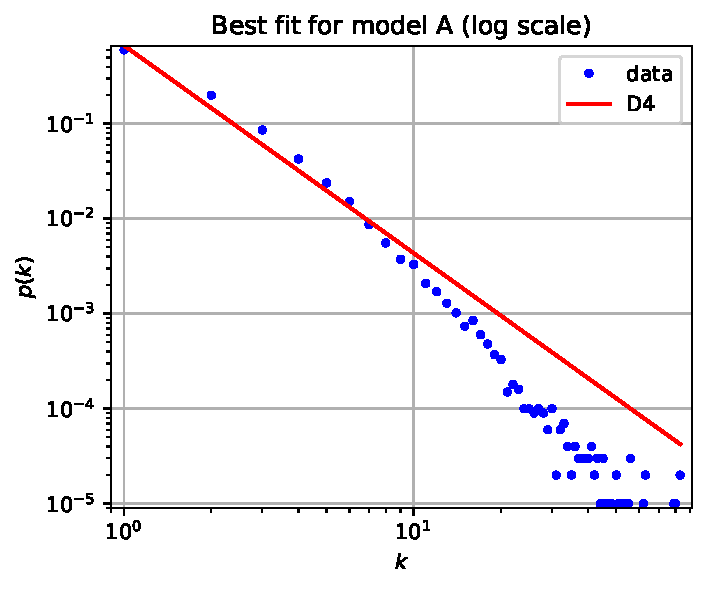
\includegraphics[width=0.45\textwidth]{modelA/best_log_dd.pdf}
		\caption{Distribution degree for model A}
		\label{fig:best_dd_A}
\end{figure}
%
\begin{figure}[H]
		\centering
		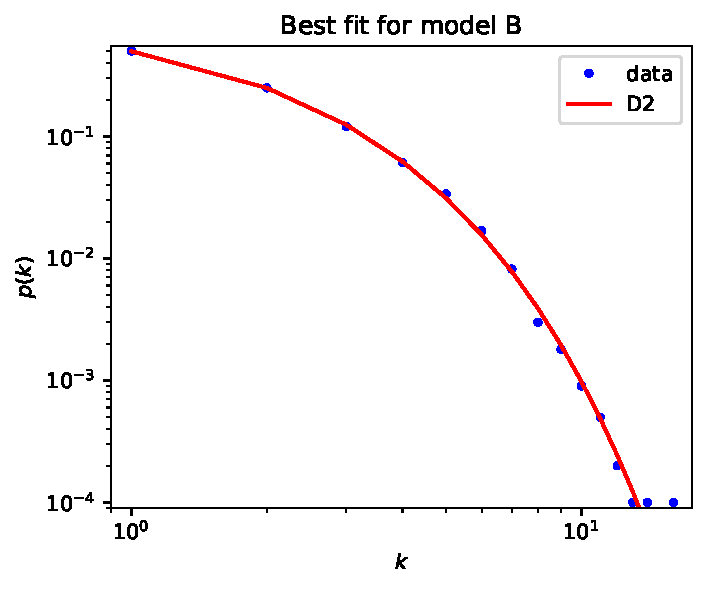
\includegraphics[width=0.45\textwidth]{modelB/best_dd.pdf}
		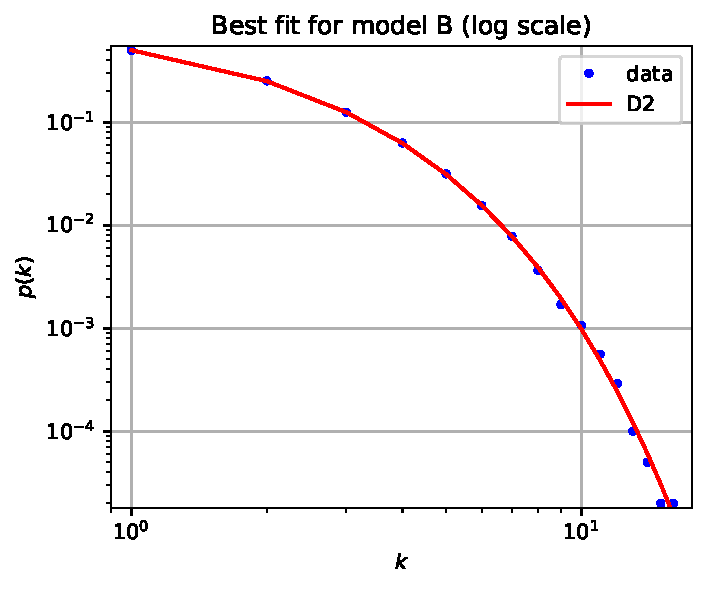
\includegraphics[width=0.45\textwidth]{modelB/best_log_dd.pdf}
		\caption{Distribution degree for model B}
		\label{fig:best_dd_B}
\end{figure}
%
\begin{figure}[H]
		\centering
		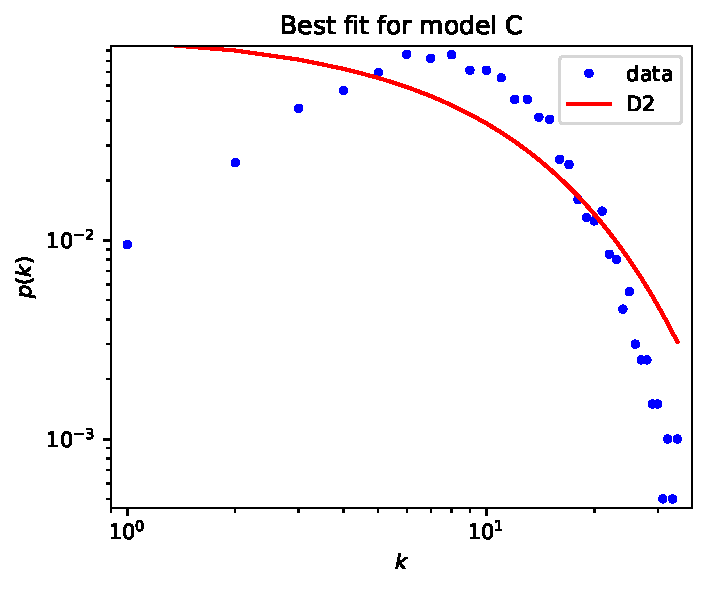
\includegraphics[width=0.45\textwidth]{modelC/best_dd.pdf}
		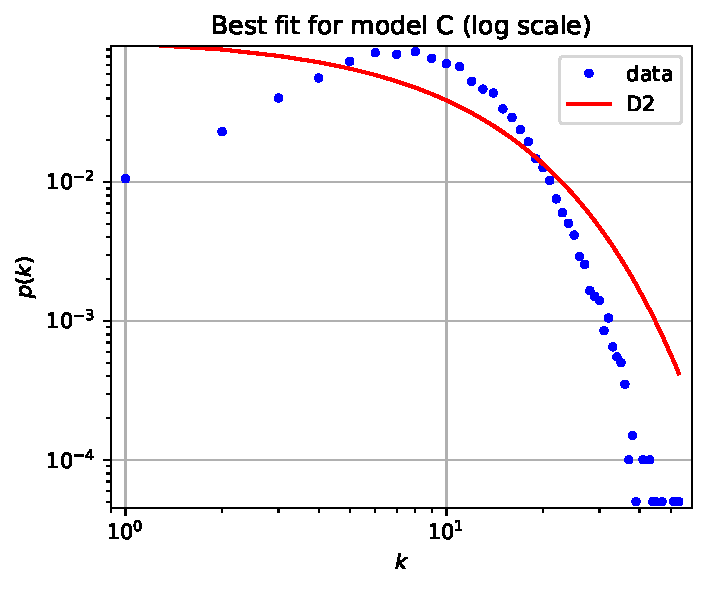
\includegraphics[width=0.45\textwidth]{modelC/best_log_dd.pdf}
		\caption{Distribution degree for model C}
		\label{fig:best_dd_C}
\end{figure}
%
\begin{figure}[H]
		\centering
		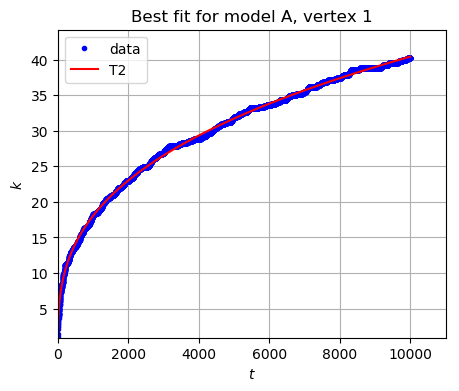
\includegraphics[width=0.45\textwidth]{modelA/best_dt1.png}
		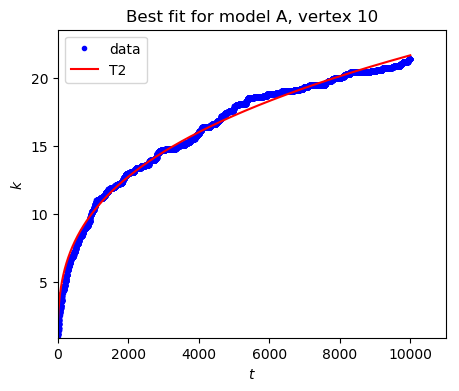
\includegraphics[width=0.45\textwidth]{modelA/best_dt10.png}
		\caption{Degree over time for model A with vertex at $t=1$ and $t=10$}
		\label{fig:best_dt1_A}
\end{figure}
%
\begin{figure}[H]
		\centering
		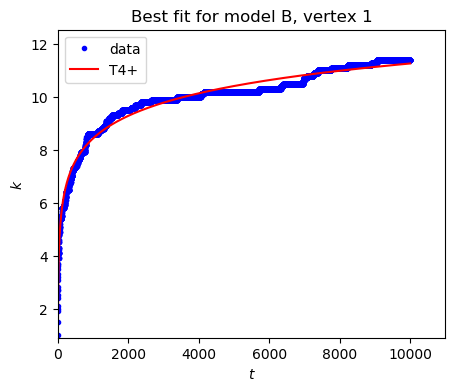
\includegraphics[width=0.45\textwidth]{modelB/best_dt1.png}
		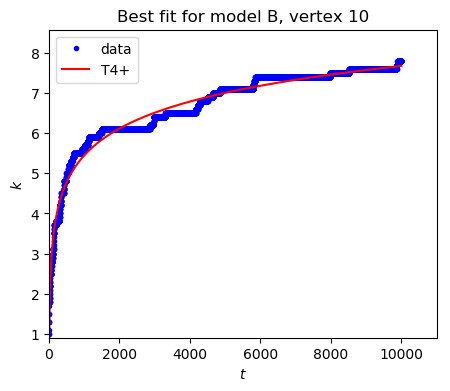
\includegraphics[width=0.45\textwidth]{modelB/best_dt10.png}
		\caption{Degree over time for model B with vertex at $t=1$ and $t=10$}
%		\label{fig:all_dd_C}
\end{figure}
%
\begin{figure}[H]
		\centering
		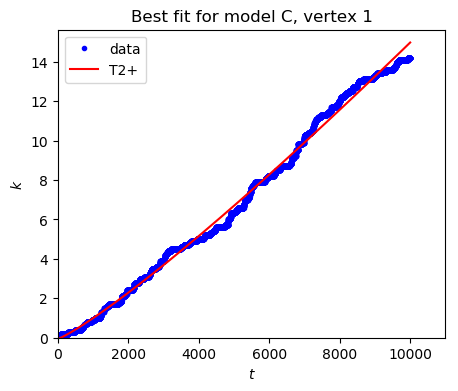
\includegraphics[width=0.45\textwidth]{modelC/best_dt1.png}
		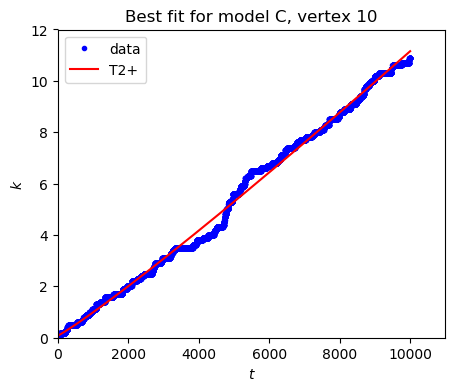
\includegraphics[width=0.45\textwidth]{modelC/best_dt10.png}
		\caption{Degree over time for model C with vertex at $t=1$ and $t=10$}
%    \label{fig:all_dd_C}
\end{figure}
%
\begin{figure}[H]
		\centering
		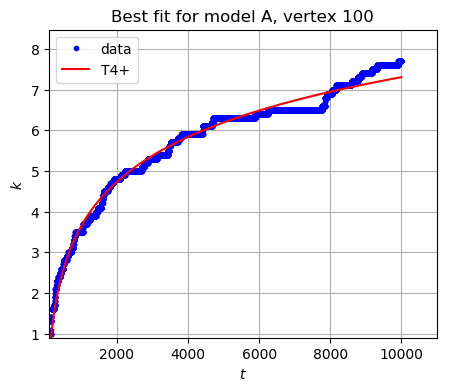
\includegraphics[width=0.45\textwidth]{modelA/best_dt100.png}
		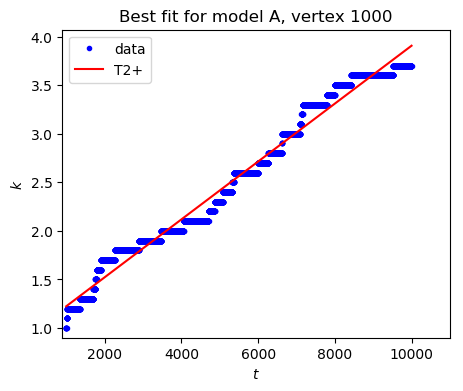
\includegraphics[width=0.45\textwidth]{modelA/best_dt1000.png}
		\caption{Degree over time for model A with vertex at $t=100$ and $t=1000$}
		\label{fig:best_dt1000_A}
\end{figure}
%
\begin{figure}[H]
		\centering
		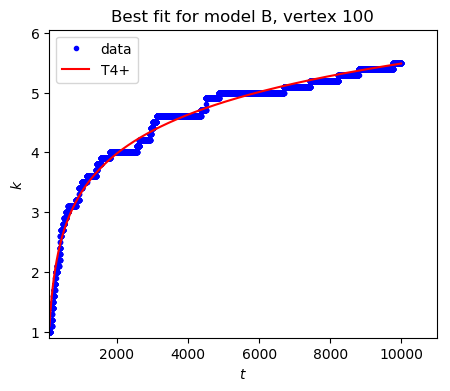
\includegraphics[width=0.45\textwidth]{modelB/best_dt100.png}
		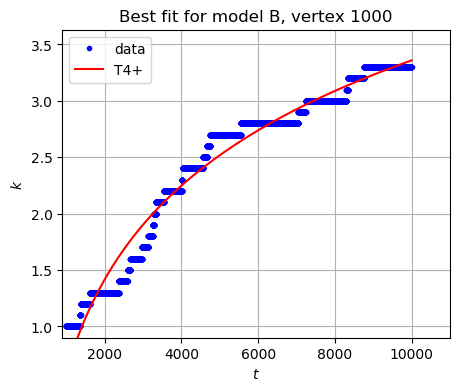
\includegraphics[width=0.45\textwidth]{modelB/best_dt1000.png}
		\caption{Degree over time for model B with vertex at $t=100$ and $t=1000$}
%    \label{fig:all_dd_C}
\end{figure}
%
\begin{figure}[H]
		\centering
		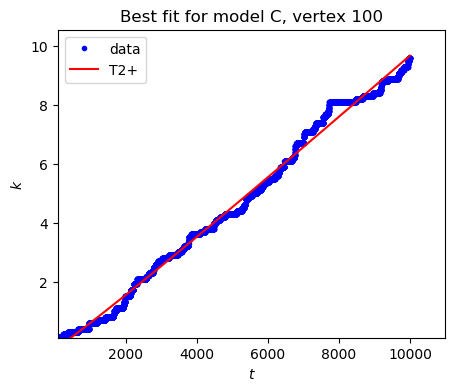
\includegraphics[width=0.45\textwidth]{modelC/best_dt100.png}
		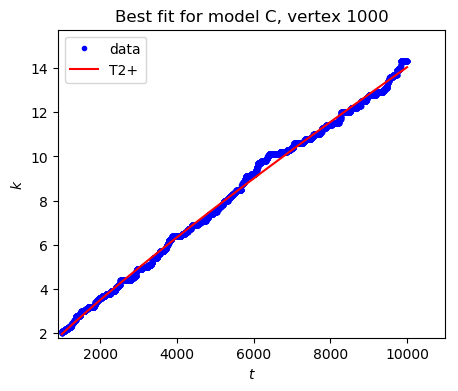
\includegraphics[width=0.45\textwidth]{modelC/best_dt1000.png}
		\caption{Degree over time for model C with vertex at $t=100$ and $t=1000$}
%    \label{fig:all_dd_C}
\end{figure}
%
\section{Discussion}

We used constant values for $m_0$ and $n_0$ for each model. We never compared 
the models with more values of $m_0$ or $n_0$ for the same model. It could have 
indicate us if the model behave differently given different graph in input. We 
could have went further and do this but we preferred to focus on the analysis of 
our different models with the input specified in the methods section.

\subsection{Model A}

% TODO Understand why we don't have this barabasi albert property %

\paragraph{Vertex degree over time}

% Check visually if k_i'(t) is about the same for every vertex chosen for the
% ranges of time the vertices coexist (make a plot).

We see in the plots~\ref{fig:best_dt1_A} to~\ref{fig:best_dt1000_A} that the 
values for $k$ of the selected vertex are very different, depending of the 
vertex chosen. If we see the value of $k$ at $t = 4000$, for the different 
graphs with $t_i$ being 1, 10, 100 and 1000, we see the values 30, 15, 6 and 2.  
It makes sense that latter vertices added to the graph have a slower grow in 
degree, as there are already some large popular vertex (with high degree), so 
the preferential attachment algorithm assigns very little probability to the new 
vertex to be selected for attachment.

% Check if the power-law dependency with 1/2 exponent gives the best fit
% to all the time series. Use model selection (lab session 3).

We checked if the power-law dependency with 1/2 exponent gives the best fit to
all the time series as required by the statement. This power-law dependency is
not always the best fit, but is close. This power-law is model T1, which has an 
AIC higher than model T2 (see tables \ref{tab:AICdt1} to \ref{tab:AICdt1000}).  
In fact the best model seems to be model T2, defined as $f(t) = at^b$, which is 
the exponential growth. It makes sense because with one free parameter we can 
better optimize this model to fit the data, by adapting $b$ to somewhat more 
close to 1/3. As we are using $m_0 = 1$, the equation 2 from session 6 is the 
same as model T1.
%
If we look at table \ref{tab:paramsdt1} to \ref{tab:paramsdt1000}, we
see that $b$ is close to $1/2$ only for $t_i = 1000$ (table 
\ref{tab:paramsdt1000}).

\paragraph{Degree distribution}

The best model for degree distribution is in the plot \ref{fig:best_dd_A}. We 
can see that the model D4 gives a pretty good approximation of the data.
%
% XXX:Homocedasticity why? We didn't checked by any maningful statistical test.
% By the non-log graph the data seems very close to the model.
%
%However, we can say that we don't have an homoscedasticity, therefore the model
%is not \textit{equally} fitting for the data for every degree k: for $k > 10$
%we are starting to loose precision with the model D5.
%
We can compare the model D4 with the others looking at table \ref{tab:AICdd} and 
the figure~\ref{fig:all_dd_A}. Model D3 is the same zeta function with parameter 
$\gamma$ fixed to 2. If we look at the table \ref{tab:params_dd} we can see that 
$\gamma = 2.189$ for model D4. It explains why D3 and D4 are not bad methods 
either. The model D5 does not converge, maybe because we are using an integer 
$k_{\max}$ parameter as real.

\subsection{Model B}

\paragraph{Vertex degree over time}

We can see again that the growth of the degree depends on the time of arrival 
For table \ref{tab:AICdt1} to \ref{tab:AICdt1000}, best model is as suggested by
the statement, the logarithmic model T4+. Indeed, we have 0 as $\Delta$ for the
vertex degree over time for this model and for every $t_i$ chosen to look at the
vertex. We can see that the model T4+ approximate really well the data looking
at figure \ref{fig:dt_B_1}, the model T4 is also very good.

\paragraph{Degree distribution}


The best model for the degree distribution for the Barabasi Albert model without
preferential attachment is the geometric one (model D2). Actually we can see
 in table
\ref{tab:AICdd}.

By looking at the figure \ref{fig:all_dd_B}, we can clearly see that
the geometric model (D2) is a really good approximation of our data. It
even goes through a lot of points of the actual data point we have until
$degree \approx 10$.

\subsection{Model C}

Following the session statement, the value of $n_0$ needs to meet $1000 \le n_0 
\le t$, so we used $n_0 = t_{\max} / 5 = 2000 $.

\paragraph{Vertex degree over time}

As expected by statement, the degree over time should fit a linear scale. By
computing the AIC and making the $\Delta$ (see tables \ref{tab:AICdt1} to
\ref{tab:AICdt1000}) we have seen that the linear model was good. Also, we are
really confident by saying it's linear when we look at the plot generated for
model C, for every $t_is$. However we find that model T0, T0+, T2 and T2+ are
the best. Model T2 is represented as $at^b$, as $b$ is close to 1 as we can see
in tables \ref{tab:AICdt1} to \ref{tab:AICdt1000}, which explain this good fit
for model T2 and T2+.

\paragraph{Degree distribution}

As we have removed the growth of the graph, the degree distribution (see 
figure~\ref{fig:all_dd_C}) no longer follows power-law distribution. As stated 
by the statement, the degree distribution for this model should be closer to a 
binomial distribution. Indeed it looks like it, but we found out it looked even 
more of a displaced Poisson with on a different scale. If we took $\lambda = 2$, 
then we would have a faster increasing and decreasing Poisson which is what we 
want. However, this Poisson has a mean of $\lambda = 2$.  Therefore, it does not 
fit our data which has a mean of approximately 10.

So we displaced the Poisson and adjusted the scale. The lasting problem was that
due do this scale and displacement, our model never produces data $\approx 0$
whereas the generated model data had a lot of values $\approx 0$.

We also made sure that the distribution giving the best fit in not a power-law,
it's looking more of a Gaussian one. However since it's not symmetric it was
hard to model the data using a normal law, for example.

In the end we chose to use a Poisson distribution as we did in session 2. It's 
not a really good fit, even the geometric one (D2) seems better. However, the 
Poisson (D1) has a $\delta$ AIC of only 726 (table \ref{tab:AICdd}). The plot of 
the geometric model can be seen in figure \ref{fig:all_dd_C} in log-scale.


\section{Methods} \label{methods}

In order to reduce noise, all the models A, B and C were run $R_{\max} = 10$ 
times.  The mean values were computed for the number of vertices of each degree, 
in the case of the degree distribution, and the mean degree for each time step.  
Finally this mean values were used for fitting by models.

For the model A and B the initial graph was an empty graph with only one vertex.  
For C we used an unconnected graph with $t_{\max}$ vertices.  Because we have no 
vertex growth, the number of vertices is constant until the end at $t = 
t_{\max}$.  For the three models we used $m_0 = 1$ as the initial number of 
edges added at each step. Changing this parameter can affect the final results, 
but was not tested.

We measured the growth of the vertex degree over time and the degree
distribution for each model. The vertex degree was measured over the time for
$t_i \in {1, 10, 100, 1000}$ successively.

We used python for generating the models, to store the results and to analyze
and plot the data. For each BA model with the letter $M$ a folder 
\texttt{data/model$M$/} contains all the results produced by this model.
Inside, for each run $0 \le R < R_{\max}$, the degree sequence is stored in the 
file \texttt{dseq\_r$R$.txt}, the degree distribution in \texttt{dd\_r$R$.txt} 
and for each $t$ in the arrival time, we produced \texttt{dt$t$\_r$R$.txt} 
tracing the degree of the vertex arriving at time $t$.

\subsection{Generating model C}

While trying to define how to make the preferential attachment for model C we
faced a problem. We were choosing from the edges to be linked to our vertex in
an array of probability $p$ (we didn't used the stubs method), with the degree
of the node over the sum of the degrees of all nodes as:
%
\begin{pycode}
p[i] = vertex.degree() / sum(graph.all_degrees())
\end{pycode}
%
However with $m_0 = 5$ and only 4 vertices  connected, we cannot choose 5
vertices, and it would not work. To mimic the stub solution, we added one
virtual degree to each unconnected node. Therefore our array of probability $p$
was computed as:
%
\begin{pycode}
if vertex.degree == 0:
	p[i] = 1 / sum(graph.all_degrees()) + sum(number_of_nodes_with_degree_0)
else:
	p[i] = vertex.degree() / (sum(graph.all_degrees()) +
		sum(number_of_nodes_with_degree_0))
\end{pycode}
%
In the end the probability vector was computed from the number of stubs.
%
\subsection{Execution}
%
In order to run the generator of models, the file \texttt{sim.py} populates the 
data from a fixed seed, so it should be reproducible. Then the two programs 
\texttt{fit\_dd.py} and \texttt{fit\_dt.py} perform the fit for the degree 
distribution and degree over time models, as well as the tables and figures 
needed in the report.

A Makefile takes care of the building process, so a simple \texttt{make} should 
be enough to build the data and run the models, as well as updating the report.

%
%
\appendix
\section{Tables}

% AICs

\begin{table}[H]
	\centering
	\begin{tabular}{rrrr}
\toprule
     &        A &        B &        C \\
\midrule
   1 & \num{7245.741} & \num{1308.885} &  \num{776.040} \\
   2 & \num{1097.608} &    \num{0.000} &    \num{0.000} \\
   3 &  \num{606.012} & \num{2505.972} & \num{6112.841} \\
   4 &  \num{359.648} & \num{2456.367} & \num{6110.839} \\
   5 &    \num{0.000} & \num{1899.960} & \num{5988.746} \\
\bottomrule
\end{tabular}
	\caption{$\Delta$ for the degree distribution.}
	\label{tab:AICdd}
\end{table}
\begin{table}[H]
	\centering
	\begin{tabular}{lrrr}
\toprule
     &         1 &         2 &         3 \\
\midrule
 0   & \num{69534.390} & \num{59969.865} & \num{10786.775} \\
 1   & \num{45188.426} & \num{48383.218} & \num{38204.833} \\
 2   &     \num{0.000} &  \num{4088.919} &    \num{33.872} \\
 3   & \num{57486.358} & \num{23686.609} & \num{65632.205} \\
 4   & \num{57130.622} &    \num{10.271} & \num{49999.142} \\
 0+  & \num{45767.062} & \num{22835.391} &  \num{4019.623} \\
 1+  & \num{27730.356} & \num{25665.773} & \num{26144.944} \\
 2+  & \num{19115.101} & \num{10442.574} &     \num{0.000} \\
 3+  &  $\infty$    &  $\infty$    &  $\infty$    \\
 4+  & \num{12117.889} &     \num{0.000} &  \num{9608.871} \\
\bottomrule
\end{tabular}
	\caption{$\Delta$ for the vertex degree over time for $t_i = 1$.}
	\label{tab:AICdt1}
\end{table}
\begin{table}[H]
	\centering
	\begin{tabular}{lrrr}
\toprule
     &         1 &         2 &         3 \\
\midrule
 0   & \num{56219.491} & \num{56948.832} &  \num{3294.824} \\
 1   & \num{33958.147} & \num{44276.525} & \num{35679.447} \\
 2   &  \num{5638.288} &  \num{4262.024} &    \num{77.463} \\
 3   & \num{80808.086} & \num{75603.323} & \num{65467.831} \\
 4   & \num{41881.941} &  \num{5870.707} & \num{48564.528} \\
 0+  & \num{33417.747} & \num{22409.635} &  \num{1463.430} \\
 1+  & \num{17922.167} & \num{15043.736} & \num{23894.852} \\
 2+  & \num{11109.884} &  \num{9443.397} &     \num{0.000} \\
 3+  &  $\infty$    &  $\infty$    &  $\infty$    \\
 4+  &     \num{0.000} &     \num{0.000} &  \num{4786.908} \\
\bottomrule
\end{tabular}
	\caption{$\Delta$ for the vertex degree over time for $t_i = 10$.}
	\label{tab:AICdt10}
\end{table}
\begin{table}[H]
	\centering
	\begin{tabular}{lrrr}
\toprule
     &         A &         B &         C \\
\midrule
 0   & \num{46992.180} & \num{56158.051} &  \num{6775.516} \\
 1   & \num{26745.892} & \num{40993.239} & \num{34445.263} \\
 2   &  \num{4084.008} & \num{11373.071} &  \num{1083.024} \\
 3   & \num{70608.550} & \num{76491.996} & \num{62248.713} \\
 4   & \num{30090.842} & \num{24884.091} & \num{46399.114} \\
 0+  & \num{22011.767} & \num{27947.947} &   \num{343.071} \\
 1+  & \num{10879.865} & \num{20065.047} & \num{20084.117} \\
 2+  &  \num{3419.044} & \num{14228.805} &     \num{0.000} \\
 3+  &  $\infty$    &  $\infty$    &  $\infty$    \\
 4+  &     \num{0.000} &     \num{0.000} &  \num{1983.962} \\
\bottomrule
\end{tabular}
	\caption{$\Delta$ for the vertex degree over time for $t_i = 100$.}
	\label{tab:AICdt100}
\end{table}
\begin{table}[H]
	\centering
	\begin{tabular}{lrrr}
\toprule
     &         1 &         2 &         3 \\
\midrule
 0   & \num{24212.569} & \num{24852.123} & \num{16241.758} \\
 1   &  \num{8639.541} &  \num{4706.668} & \num{35197.595} \\
 2   &  \num{4130.729} &  \num{4019.593} &   \num{465.222} \\
 3   & \num{58036.196} & \num{55068.283} & \num{69970.214} \\
 4   & \num{31443.880} & \num{27424.662} & \num{49730.948} \\
 0+  &     \num{0.021} & \num{10189.872} &  \num{2862.488} \\
 1+  &  \num{5672.115} &  \num{3420.122} & \num{13800.604} \\
 2+  &     \num{0.000} &  \num{1158.596} &   \num{424.130} \\
 3+  &  $\infty$    &  $\infty$    &  $\infty$    \\
 4+  &   \num{159.748} &     \num{0.000} &     \num{0.000} \\
\bottomrule
\end{tabular}
	\caption{$\Delta$ for the vertex degree over time for $t_i = 1000$.}
	\label{tab:AICdt1000}
\end{table}

% Params
\begin{table}[H]
	\centering
	\begin{tabular}{lrrr}
\toprule
 Dataset        &      1 &      2 &      3 \\
\midrule
 $1_{\lambda}$  &  \num{1.593} &  \num{1.593} & \num{10.000} \\
 $2_{q}$        &  \num{0.500} &  \num{0.500} &  \num{0.100} \\
 $4_{\gamma}$   &  \num{2.189} &  \num{2.078} &  \num{2.000} \\
 $5_{\gamma}$   &  \num{2.000} &  \num{2.000} &  \num{2.000} \\
 $5_{k_{\max}}$ & \num{20.000} & \num{20.000} & \num{20.000} \\
\bottomrule
\end{tabular}
	\caption{Parameters for degree distribution models fitting.}
	\label{tab:param_dd}
\end{table}
\begin{table}[H]
	\centering
	\begin{tabular}{lrrr}
\toprule
 Dataset   &       A &       B &         C \\
\midrule
 $0 a$     &   \num{0.005} &   \num{0.002} &     \num{0.001} \\
 $1 a$     &   \num{0.434} &   \num{0.134} &     \num{0.110} \\
 $2 a$     &   \num{1.616} &   \num{3.348} &     \num{0.000} \\
 $2 b$     &   \num{0.350} &   \num{0.133} &     \num{1.166} \\
 $3 a$     &  \num{14.000} &   \num{8.637} &    \num{-0.000} \\
 $3 c$     &   \num{0.000} &   \num{0.000} &    \num{-0.527} \\
 $4 a$     &   \num{3.792} &   \num{1.222} &     \num{0.837} \\
 $4 d_1$   &  \num{-0.849} &   \num{1.117} &    \num{-0.871} \\
 $0+ a$    &   \num{0.003} &   \num{0.000} &     \num{0.002} \\
 $0+ d$    &  \num{14.000} &   \num{8.496} &    \num{-0.735} \\
 $1+ a$    &   \num{0.370} &   \num{0.072} &     \num{0.178} \\
 $1+ d$    &   \num{5.000} &   \num{5.000} &    \num{-5.000} \\
 $2+ a$    &   \num{0.500} &   \num{0.413} &     \num{0.000} \\
 $2+ b$    &   \num{0.466} &   \num{0.300} &     \num{1.155} \\
 $2+ d$    &   \num{5.000} &   \num{5.000} &    \num{-0.058} \\
 $3+ a$    &   \num{0.289} &   \num{0.289} &     \num{0.289} \\
 $3+ c$    &   \num{0.853} &   \num{0.853} &     \num{0.853} \\
 $3+ d$    & \num{-10.000} & \num{-10.000} &   \num{-10.000} \\
 $4+ a$    &  \num{12.971} &   \num{1.230} &    \num{48.860} \\
 $4+ d_1$  & \num{952.161} &   \num{1.413} & \num{27177.319} \\
 $4+ d_2$  & \num{-80.698} &  \num{-0.060} &  \num{-500.000} \\
\bottomrule
\end{tabular}
	\caption{Parameters for the vertex degree over time for $t_i = 1$.}
	\label{tab:paramsdt1}
\end{table}
\begin{table}[H]
	\centering
	\begin{tabular}{lrrr}
\toprule
 Param        &       A &       B &       C \\
\midrule
 $T0$, $a$    &   \num{0.003} &   \num{0.001} &   \num{0.001} \\
 $T1$, $a$    &   \num{0.237} &   \num{0.093} &   \num{0.087} \\
 $T2$, $a$    &   \num{1.036} &   \num{1.795} &   \num{0.001} \\
 $T2$, $b$    &   \num{0.330} &   \num{0.159} &   \num{1.070} \\
 $T3$, $a$    &  \num{-0.330} &  \num{-0.331} &  \num{-0.352} \\
 $T3$, $c$    &  \num{-1.363} &  \num{-1.363} &  \num{-0.566} \\
 $T4$, $a$    &   \num{2.079} &   \num{0.820} &   \num{0.693} \\
 $T4$, $d_1$  &  \num{-9.843} &  \num{-9.408} &  \num{-9.875} \\
 $T0+$, $a$   &   \num{0.001} &   \num{0.000} &   \num{0.001} \\
 $T0+$, $d$   &  \num{10.366} &   \num{5.424} &  \num{-0.220} \\
 $T1+$, $a$   &   \num{0.172} &   \num{0.036} &   \num{0.139} \\
 $T1+$, $d$   &   \num{4.885} &   \num{4.303} &  \num{-3.958} \\
 $T2+$, $a$   &   \num{0.800} &   \num{0.314} &   \num{0.000} \\
 $T2+$, $b$   &   \num{0.355} &   \num{0.300} &   \num{1.088} \\
 $T2+$, $d$   &   \num{0.798} &   \num{2.893} &   \num{0.076} \\
 $T3+$, $a$   &   \num{0.289} &   \num{0.289} &   \num{0.289} \\
 $T3+$, $c$   &   \num{0.853} &   \num{0.853} &   \num{0.853} \\
 $T3+$, $d$   & \num{-10.000} & \num{-10.000} & \num{-10.000} \\
 $T4+$, $a$   &   \num{3.238} &   \num{0.970} &   \num{1.874} \\
 $T4+$, $d_1$ &  \num{-8.242} &  \num{-1.528} &  \num{11.972} \\
 $T4+$, $d_2$ & \num{-10.000} &  \num{-1.258} & \num{-10.000} \\
\bottomrule
\end{tabular}
	\caption{Parameters for the vertex degree over time for $t_i = 10$.}
	\label{tab:paramsdt10}
\end{table}
\begin{table}[H]
	\centering
	\begin{tabular}{lrrr}
\toprule
 Param        &       A &       B &       C \\
\midrule
 $T0$, $a$    &   \num{0.001} &   \num{0.001} &   \num{0.001} \\
 $T1$, $a$    &   \num{0.083} &   \num{0.064} &   \num{0.074} \\
 $T2$, $a$    &   \num{0.422} &   \num{0.735} &   \num{0.000} \\
 $T2$, $b$    &   \num{0.313} &   \num{0.220} &   \num{1.122} \\
 $T3$, $a$    &  \num{-0.500} &  \num{-0.500} &  \num{-0.500} \\
 $T3$, $c$    &  \num{-0.500} &  \num{-0.500} &  \num{-0.500} \\
 $T4$, $a$    &   \num{0.718} &   \num{0.563} &   \num{0.568} \\
 $T4$, $d_1$  & \num{-15.000} & \num{-15.000} & \num{-15.000} \\
 $T0+$, $a$   &   \num{0.000} &   \num{0.000} &   \num{0.001} \\
 $T0+$, $d$   &   \num{3.674} &   \num{3.410} &  \num{-0.463} \\
 $T1+$, $a$   &   \num{0.059} &   \num{0.033} &   \num{0.128} \\
 $T1+$, $d$   &   \num{1.864} &   \num{2.366} &  \num{-4.056} \\
 $T2+$, $a$   &   \num{0.498} &   \num{0.289} &   \num{0.001} \\
 $T2+$, $b$   &   \num{0.300} &   \num{0.300} &   \num{1.047} \\
 $T2+$, $d$   &  \num{-0.328} &   \num{1.054} &  \num{-0.304} \\
 $T3+$, $a$   &   \num{0.289} &   \num{0.289} &   \num{0.289} \\
 $T3+$, $c$   &   \num{0.853} &   \num{0.853} &   \num{0.853} \\
 $T3+$, $d$   & \num{-10.000} & \num{-10.000} & \num{-10.000} \\
 $T4+$, $a$   &   \num{1.614} &   \num{0.931} &   \num{1.757} \\
 $T4+$, $d_1$ &  \num{50.000} & \num{-10.000} & \num{-10.000} \\
 $T4+$, $d_2$ &  \num{-7.569} &  \num{-3.089} & \num{-10.000} \\
\bottomrule
\end{tabular}
	\caption{Parameters for the vertex degree over time for $t_i = 100$.}
	\label{tab:paramsdt100}
\end{table}
\begin{table}[H]
	\centering
	\begin{tabular}{lrrr}
\toprule
 Dataset   &         A &       B &         C \\
\midrule
 $0 a$     &     \num{0.000} &   \num{0.000} &     \num{0.001} \\
 $1 a$     &     \num{0.036} &   \num{0.034} &     \num{0.120} \\
 $2 a$     &     \num{0.016} &   \num{0.025} &     \num{0.005} \\
 $2 b$     &     \num{0.596} &   \num{0.537} &     \num{0.864} \\
 $3 a$     &    \num{-0.500} &  \num{-0.500} &    \num{-0.500} \\
 $3 c$     &    \num{-0.500} &  \num{-0.500} &    \num{-0.500} \\
 $4 a$     &     \num{0.306} &   \num{0.300} &     \num{1.013} \\
 $4 d_1$   &   \num{-15.000} & \num{-15.000} &   \num{-15.000} \\
 $0+ a$    &     \num{0.000} &   \num{0.000} &     \num{0.001} \\
 $0+ d$    &     \num{0.925} &   \num{1.003} &     \num{0.928} \\
 $1+ a$    &     \num{0.041} &   \num{0.037} &     \num{0.183} \\
 $1+ d$    &    \num{-0.360} &  \num{-0.224} &    \num{-4.921} \\
 $2+ a$    &     \num{0.000} &   \num{0.334} &     \num{0.004} \\
 $2+ b$    &     \num{1.001} &   \num{0.300} &     \num{0.880} \\
 $2+ d$    &     \num{0.926} &  \num{-1.835} &     \num{0.132} \\
 $3+ a$    &     \num{0.289} &   \num{0.289} &     \num{0.289} \\
 $3+ c$    &     \num{0.853} &   \num{0.853} &     \num{0.853} \\
 $3+ d$    &   \num{-10.000} & \num{-10.000} &   \num{-10.000} \\
 $4+ a$    &    \num{16.509} &   \num{1.460} &    \num{48.389} \\
 $4+ d_1$  & \num{50000.000} & \num{743.241} & \num{31025.620} \\
 $4+ d_2$  &  \num{-177.765} & \num{-10.149} &  \num{-500.000} \\
\bottomrule
\end{tabular}
	\caption{Parameters for the vertex degree over time for $t_i = 1000$.}
	\label{tab:paramsdt1000}
\end{table}

\newpage
\section{Figures with all models}

\begin{figure}[H]
		\centering
		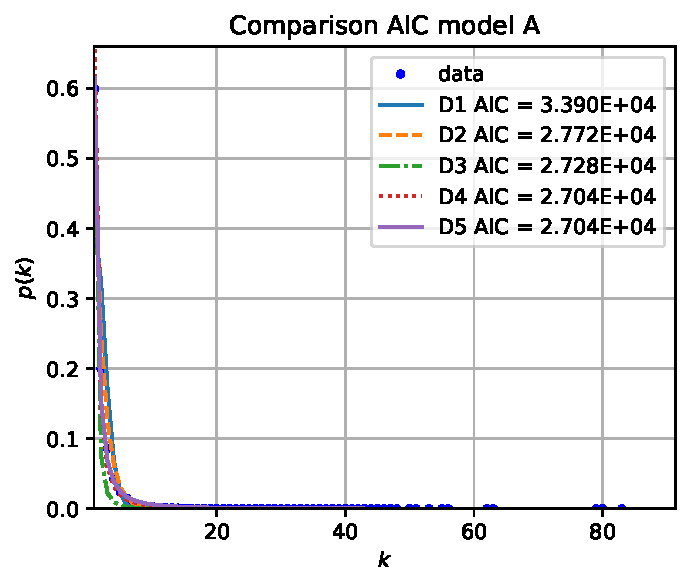
\includegraphics[width=0.45\textwidth]{modelA/all_dd.pdf}
		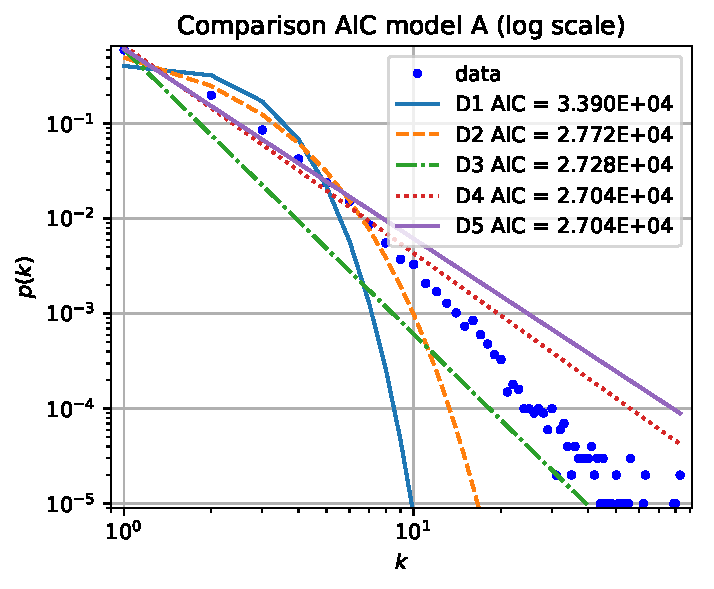
\includegraphics[width=0.45\textwidth]{modelA/all_log_dd.pdf}
		\caption{Distribution degree for model A}
		\label{fig:all_dd_A}
\end{figure}
%
\begin{figure}[H]
		\centering
		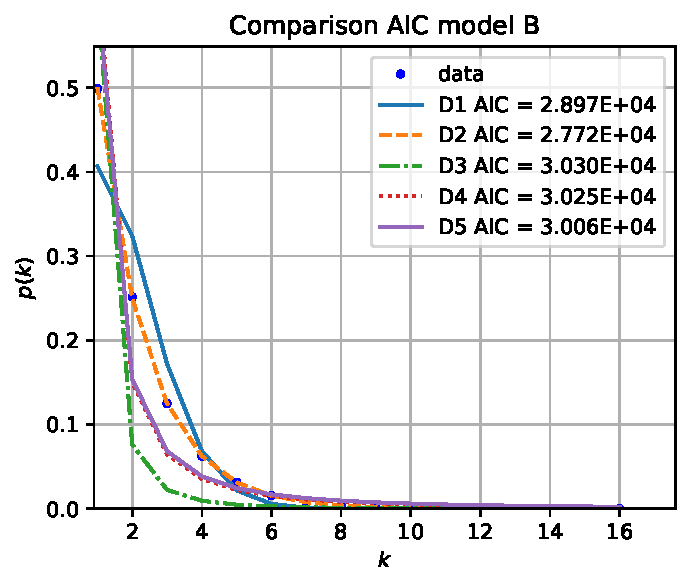
\includegraphics[width=0.45\textwidth]{modelB/all_dd.pdf}
		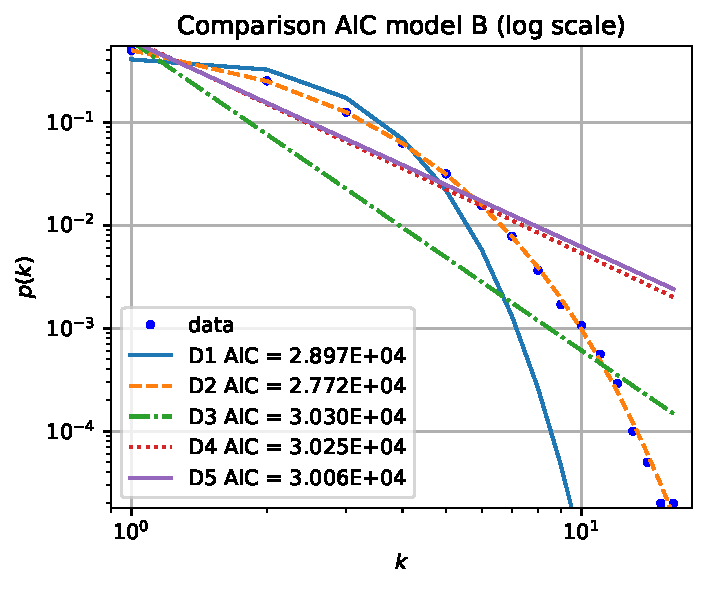
\includegraphics[width=0.45\textwidth]{modelB/all_log_dd.pdf}
		\caption{Distribution degree for model B}
		\label{fig:all_dd_B}
\end{figure}
%
\begin{figure}[H]
		\centering
		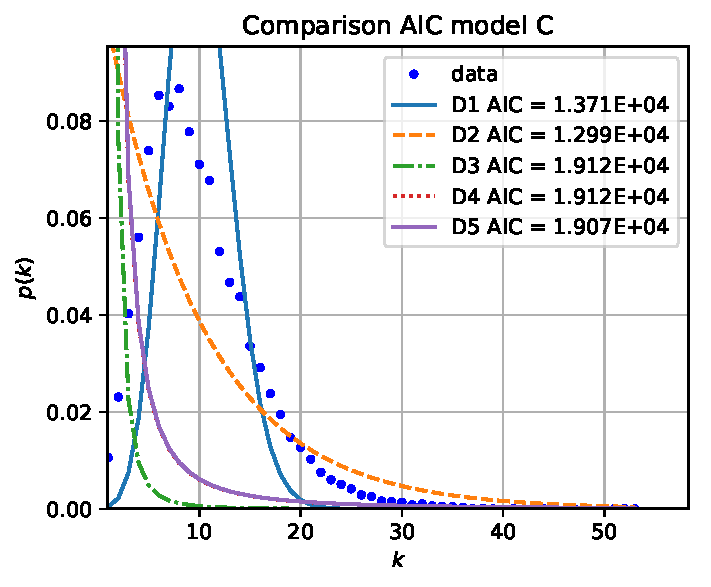
\includegraphics[width=0.45\textwidth]{modelC/all_dd.pdf}
		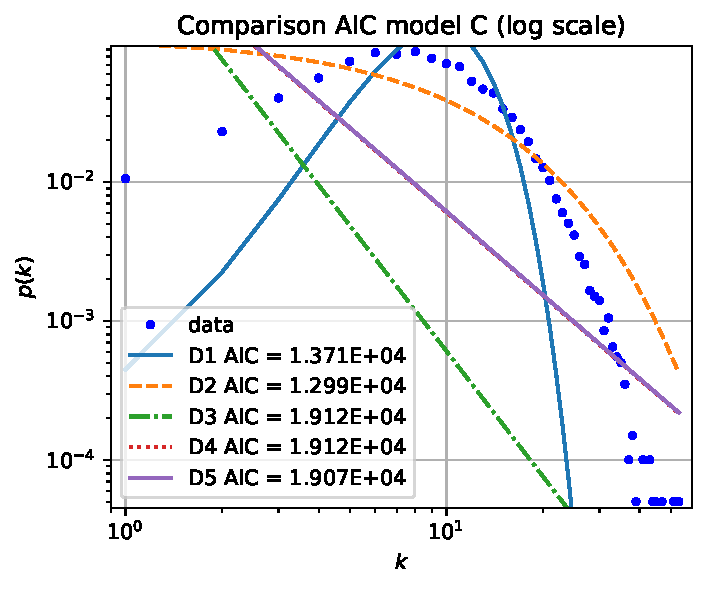
\includegraphics[width=0.45\textwidth]{modelC/all_log_dd.pdf}
		\caption{Distribution degree for model C}
		\label{fig:all_dd_C}
\end{figure}
%
\begin{figure}[H]
    \centering
		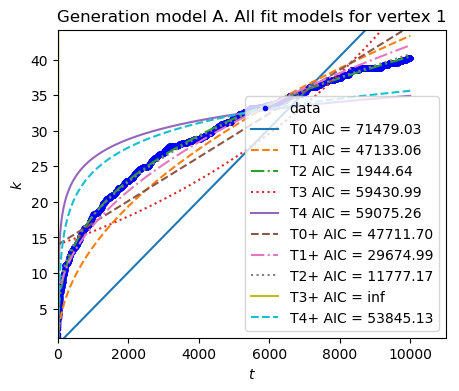
\includegraphics[width=0.45\textwidth]{modelA/all_dt1.png}
		\caption{Degree over time for model A with vertex at $t=1$}
%		\label{fig:all_dd_C}
\end{figure}
%
\begin{figure}[H]
    \centering
		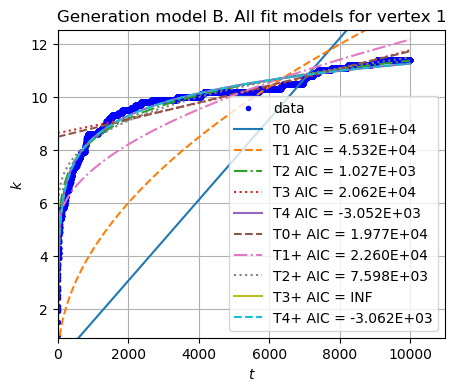
\includegraphics[width=0.45\textwidth]{modelB/all_dt1.png}
		\caption{Degree over time for model B with vertex at $t=1$}
%		\label{fig:all_dd_C}
\end{figure}
%
\begin{figure}[H]
		\centering
		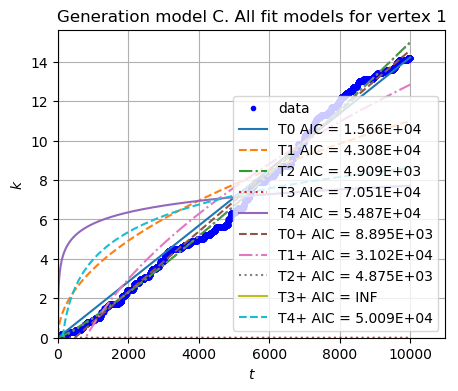
\includegraphics[width=0.45\textwidth]{modelC/all_dt1.png}
		\caption{Degree over time for model C with vertex at $t=1$}
%    \label{fig:all_dd_C}
\end{figure}
%
\begin{figure}[H]
    \centering
		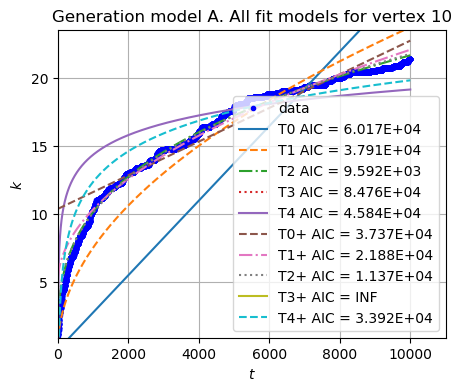
\includegraphics[width=0.45\textwidth]{modelA/all_dt10.png}
		\caption{Degree over time for model A with vertex at $t=10$}
%		\label{fig:all_dd_C}
\end{figure}
%
\begin{figure}[H]
    \centering
		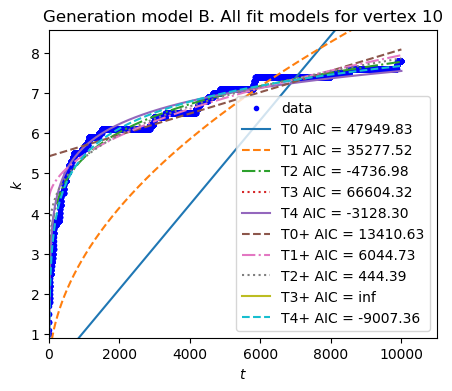
\includegraphics[width=0.45\textwidth]{modelB/all_dt10.png}
		\caption{Degree over time for model B with vertex at $t=10$}
%		\label{fig:all_dd_C}
\end{figure}
%
\begin{figure}[H]
		\centering
		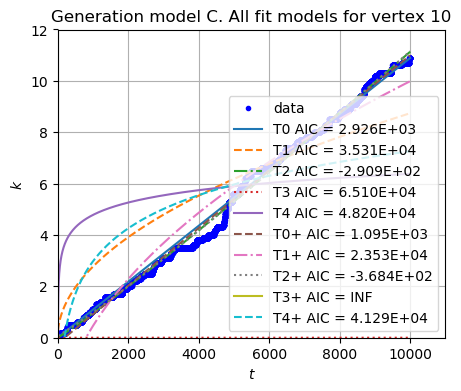
\includegraphics[width=0.45\textwidth]{modelC/all_dt10.png}
		\caption{Degree over time for model C with vertex at $t=10$}
%		\label{fig:all_dd_C}
\end{figure}
%
\begin{figure}[H]
    \centering
		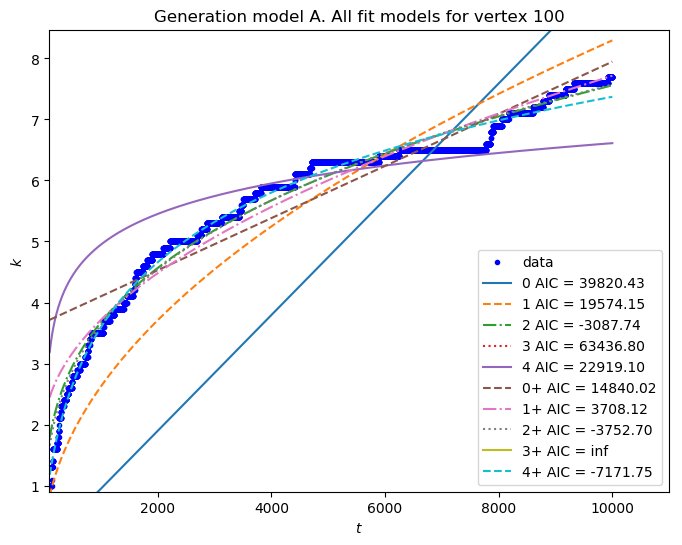
\includegraphics[width=0.45\textwidth]{modelA/all_dt100.png}
		\caption{Degree over time for model A with vertex at $t=100$}
%    \label{fig:all_dd_C}
\end{figure}
%
\begin{figure}[H]
    \centering
		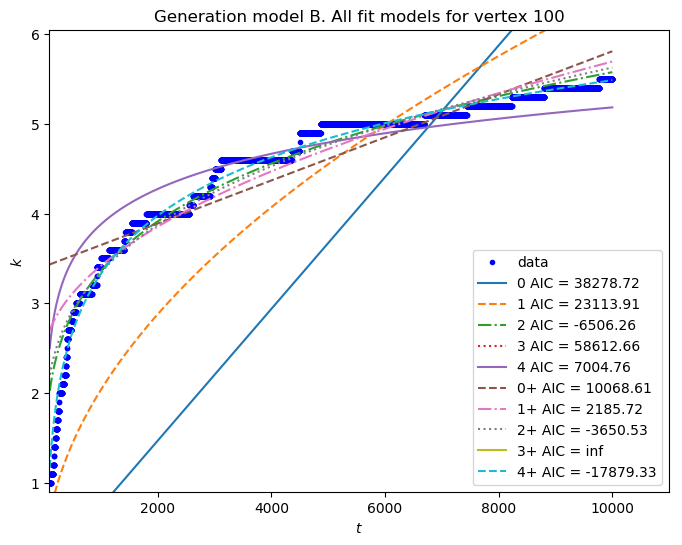
\includegraphics[width=0.45\textwidth]{modelB/all_dt100.png}
		\caption{Degree over time for model B with vertex at $t=100$}
%    \label{fig:all_dd_C}
\end{figure}
%
\begin{figure}[H]
		\centering
		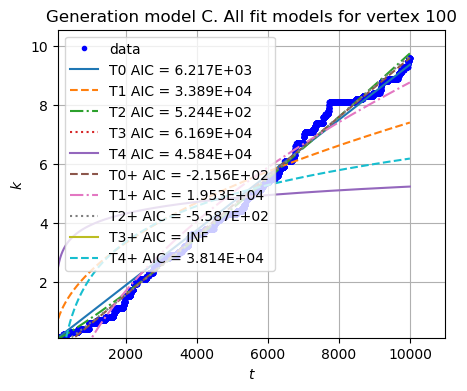
\includegraphics[width=0.45\textwidth]{modelC/all_dt100.png}
		\caption{Degree over time for model C with vertex at $t=100$}
%    \label{fig:all_dd_C}
\end{figure}
%
\begin{figure}[H]
    \centering
		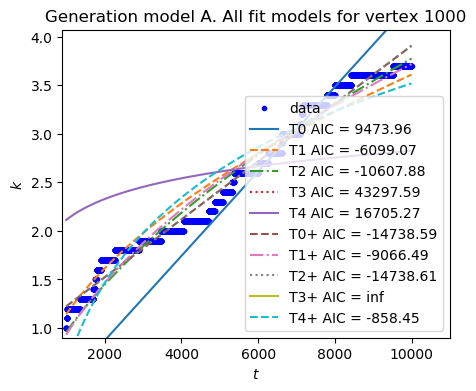
\includegraphics[width=0.45\textwidth]{modelA/all_dt1000.png}
		\caption{Degree over time for model A with vertex at $t=10000$}
%		\label{fig:all_dd_C}
\end{figure}
%
\begin{figure}[H]
    \centering
		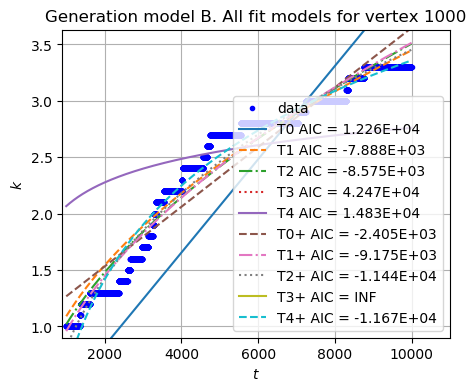
\includegraphics[width=0.45\textwidth]{modelB/all_dt1000.png}
		\caption{Degree over time for model B with vertex at $t=1000$}
%    \label{fig:all_dd_C}
\end{figure}
%
\begin{figure}[H]
		\centering
		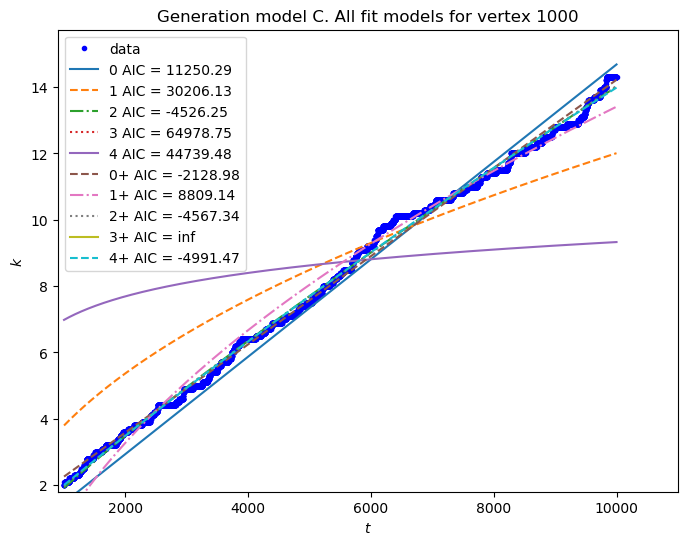
\includegraphics[width=0.45\textwidth]{modelC/all_dt1000.png}
		\caption{Degree over time for model C with vertex at $t=1000$}
		\label{fig:allC_dt1000}
\end{figure}

\end{document}
